
\subsection{Organigrama}

\begin{figure}[H]
	\centering
	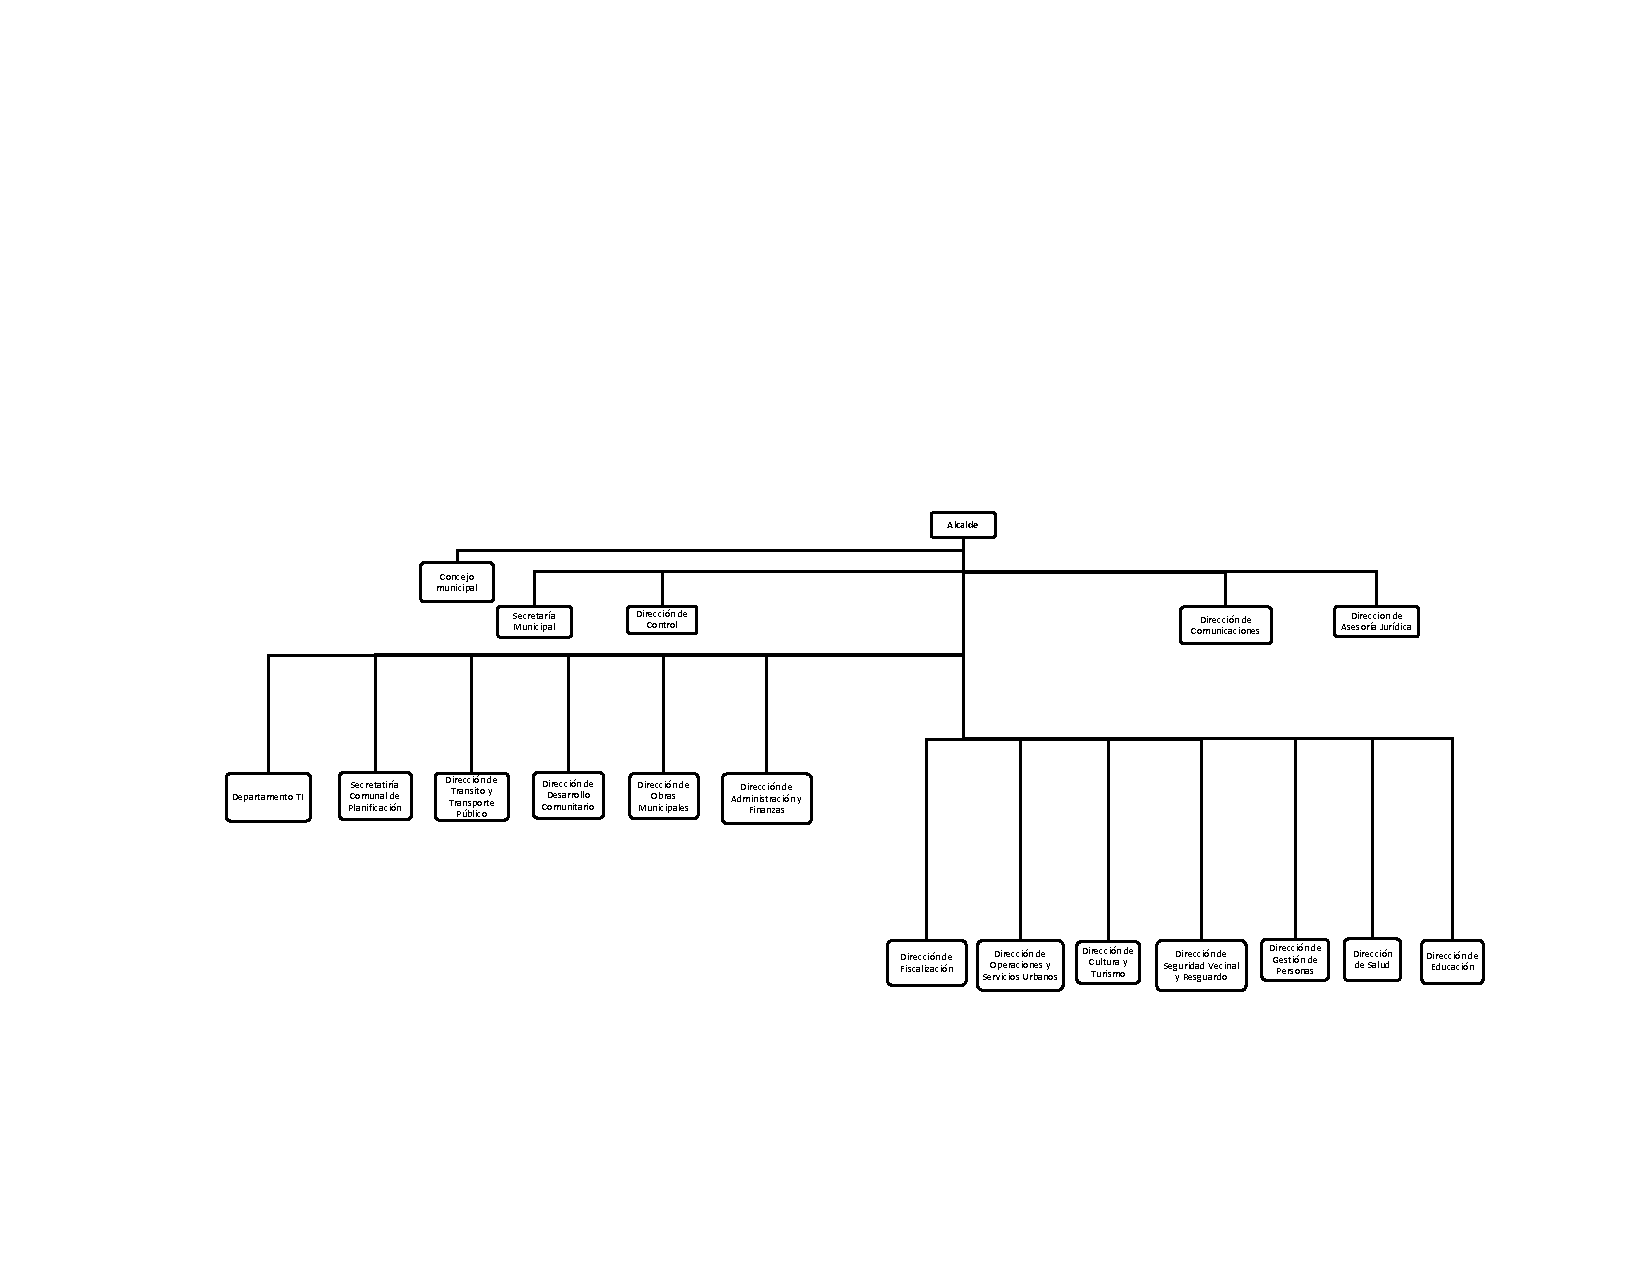
\includegraphics[width=1\textwidth]{fragments/01structure/organigramaMunicipalidad.pdf}\\
\caption{Organigrama}
\label{FIG:ORGANIGRAMA}
\end{figure}


\subsection{Rationale}
El alcance de este trabajo abarca solo las siguientes divisiones:
\begin{itemize}
	\item {
		\textbf{Departamento de asuntos municipales}. Perteneciente a la secretaría municipal. Este se compone de las siguientes oficinas:
		\begin{itemize}
			\item Oficina de partes alcaldía
			\item Sección resolutiva
			\item Sección administrativa
		\end{itemize}
	}
	\item {
		\textbf{Departamento de certificación y archivo}.  Perteneciente a la secretaría municipal. Este se compone de las siguientes oficinas:
		\begin{itemize}
			\item Oficina de registro municipal de transferencias
			\item Oficina de control de archivo y representación.
		\end{itemize}
	}
	\item {
		\textbf{Departamento de cartografía}.
	}
	\item {
		\textbf{Departamento de revisión de procesos de contratación pública}
	}
	\item {
		\textbf{Departamento de auditoría operativa}
	}
	\item {
		\textbf{Departamento Revisión de procesos de pago, bienes y servicios}
	}
\end{itemize}

Se establece para cada departamento la siguiente estructura base:
\begin{itemize}
	\item Un(a) Jefe(a) de departamento.
	\item Un(a) Secretario(a) general de departamento.
	\item Uno o más ejecutivos de departamento.
	\item Un encargado de TI del departamento.
\end{itemize}


Se establece para cada oficina la siguiente estructura base:
\begin{itemize}
	\item Un(a) Jefe(a) de oficina.
	\item Un(a) Secretario(a) general.
	\item Uno o más ejecutivos de oficina.
\end{itemize}

Se establece para cada secretaría la siguiente estructura base:
\begin{itemize}
	\item Un(a) Secretario(a) general.
	\item Uno o más ejecutivos de oficina.
\end{itemize}

